% !TeX root = main.tex
% !TeX encoding = UTF-8
% !TeX spellcheck = de_DE
% !TeX TXS-program:bibliography = txs:///biber
% =====================================================================
%  Projektarbeit (Master) – Hauptdatei
%  Layout übernommen aus der Bachelorarbeit (Knechtel-Vorlage)
%  Kompilieren: pdflatex -> biber -> pdflatex -> pdflatex
% =====================================================================

\documentclass[12pt,a4paper]{article}

% ---------------------------------------------------------------------
%  Angaben zur Arbeit – HIER ANPASSEN
% ---------------------------------------------------------------------
\newcommand{\ArbeitTyp}{Projektarbeit}
\newcommand{\ArbeitTitel}{Theoretische Betrachtung zu Nano-Imprint-Lithographie}
\newcommand{\ArbeitUntertitel}{New-Era-Tech für großes Zeug bei X-FAB}
\newcommand{\AutorName}{Luis Marcus}
\newcommand{\AutorGeburt}{geb. am 12.08.2003 in Suhl}
\newcommand{\AutorMatrikel}{315768}
\newcommand{\Studiengang}{Elektro- und Informationstechnik}
\newcommand{\Hochschule}{Hochschule Schmalkalden}
\newcommand{\Fakultaet}{Fakultät Elektrotechnik}
\newcommand{\Referent}{Prof. Dr.-Ing. Roy Knechtel}
\newcommand{\Korreferent}{Dipl.-Ing. Holger Klingner}
\newcommand{\Firma}{X-FAB MEMS Foundry GmbH, Erfurt}
\newcommand{\FirmaKurz}{X-FAB}
\newcommand{\AbgabeOrt}{Erfurt}
\newcommand{\AbgabeDatum}{TT.MM.JJJJ}

% Logos (Ordner abbildungen/Logos/ aus der BA einfach herüberkopieren)
\newcommand{\LogoFirma}{abbildungen/Logos/X-FAB_logo_petrol_RGB_high-1333927202.jpg}
\newcommand{\LogoHochschule}{abbildungen/Logos/HSSMLogo.png}

% Sperrvermerk ein-/ausschalten
\newif\ifSperrvermerk
\Sperrvermerktrue   % \Sperrvermerkfalse, falls kein Sperrvermerk nötig

% ---------------------------------------------------------------------
% !TeX root = main.tex
% =====================================================================
%  Präambel – Pakete und Layout (wie Bachelorarbeit)
% =====================================================================

% ---------- Sprache & Schrift ----------
\usepackage[utf8]{inputenc}
\usepackage[T1]{fontenc}
\usepackage[ngerman]{babel}
\usepackage{csquotes}                 % deutsche Anführungszeichen (auch für biblatex)

% ---------- Seitenlayout nach Knechtel-Vorlage ----------
\usepackage{geometry}
\geometry{left=3cm,right=2.5cm,top=2.5cm,bottom=2.0cm}
\usepackage{setspace}
\setstretch{1.5}

\usepackage{fancyhdr}
\pagestyle{fancy}
\fancyhf{}
\fancyfoot[C]{\thepage}
% Dünne Linie oben wie in der BA. Entfernen mit:
% \renewcommand{\headrulewidth}{0pt}

% ---------- Inhaltsverzeichnis ----------
\usepackage{tocloft}
\setlength{\cftbeforesecskip}{6pt}

% ---------- Fußnoten ----------
\usepackage[bottom]{footmisc}
\interfootnotelinepenalty=10000

% ---------- Tabellen ----------
\usepackage[table]{xcolor}            % lädt auch colortbl
\usepackage{array}
\usepackage{tabularx}
\usepackage{booktabs}
\newcolumntype{L}[1]{>{\raggedright\arraybackslash}p{#1}}
\newcolumntype{C}[1]{>{\centering\arraybackslash}p{#1}}

% ---------- Abbildungen ----------
\usepackage{graphicx}
\graphicspath{{./abbildungen/}}
\usepackage{float}
\usepackage{caption}
\usepackage{subcaption}
\usepackage{adjustbox}
\usepackage[percent]{overpic}
\usepackage{pdfpages}
\usepackage{pdflscape}
\usepackage{pgfplots}
\pgfplotsset{compat=1.18}

% ---------- Mathematik & Einheiten ----------
\usepackage{amsmath,amssymb}
\usepackage{siunitx}
\sisetup{locale=DE, per-mode=symbol}
\DeclareSIUnit{\kilogramforce}{kgf}

% ---------- Listen ----------
\usepackage{enumitem}
\setlist[itemize]{noitemsep, topsep=0pt}

% ---------- Sonstiges ----------
\usepackage{comment}

% Silbentrennung für Problemwörter, z. B.:
% \hyphenation{Wieder-holbar-keits}

% ---------- Quellcode ----------
\usepackage{listings}
\lstset{
	language=Python,
	basicstyle=\ttfamily\small,
	keywordstyle=\color{blue},
	commentstyle=\color{gray},
	stringstyle=\color{green!50!black},
	numbers=left,
	numberstyle=\tiny,
	breaklines=true,
	frame=single
}

% ---------- Literatur ----------
\usepackage[backend=biber]{biblatex}
\addbibresource{literatur.bib}

% ---------- Hyperref (möglichst zuletzt laden) ----------
\usepackage{hyperref}
% Für eine Druckversion ohne farbige Linkrahmen: \hypersetup{hidelinks}
\hypersetup{
	pdftitle={\ArbeitTitel},
	pdfauthor={\AutorName}
}

% ---------------------------------------------------------------------

\newcounter{SeiteVorspann}   % merkt sich die römische Seitenzahl

\begin{document}

% ========== Deckblatt ==========
\pagenumbering{alph}          % unsichtbar, vermeidet doppelte PDF-Seitenanker
% !TeX root = ../main.tex
% ========== Deckblatt ==========
\begin{titlepage}
	\begin{spacing}{1.5}
		\thispagestyle{empty}
		\centering

		% Logos nebeneinander (Platzhalter, falls Datei fehlt)
		\begin{minipage}{0.49\textwidth}
			\flushleft
			\IfFileExists{\LogoFirma}
				{\includegraphics[width=4cm]{\LogoFirma}}
				{\fbox{\parbox[c][1.5cm][c]{4cm}{\centering Logo Firma}}}
		\end{minipage}
		\begin{minipage}{0.49\textwidth}
			\flushright
			\IfFileExists{\LogoHochschule}
				{\includegraphics[width=6cm]{\LogoHochschule}}
				{\fbox{\parbox[c][1.5cm][c]{6cm}{\centering Logo Hochschule}}}
		\end{minipage}

		\vspace{1.5cm}

		% Art der Arbeit
		\Hochschule\\
		\Fakultaet\\[1.0cm]
		{\large \ArbeitTyp\\[0.5cm]}

		% Titel
		{\Large\textbf{\ArbeitTitel}\\[0.3cm]}
		{\large \ArbeitUntertitel\\[1.0cm]}

		% Verfasser
		vorgelegt von\\[0.5cm]
		{\Large\textbf{\AutorName}}\\
		\AutorGeburt\\
		Matrikelnummer: \AutorMatrikel\\[1.0cm]

		im Studiengang \Studiengang\\[1cm]

		% Bei Bedarf (z. B. für die Masterarbeit) wieder einkommentieren:
		% zur\\
		% Erlangung des akademischen Grades\\
		% Master of Science\\[1cm]

		Referent: \Referent\\
		Korreferent: \Korreferent\\[1cm]
		\AbgabeOrt, den \AbgabeDatum

		\vfill
	\end{spacing}
\end{titlepage}


% ========== Vorspann (römische Seitenzahlen) ==========
\newpage
\pagenumbering{Roman}
\ifSperrvermerk
	% !TeX root = ../main.tex
% ========== Sperrvermerk ==========
% Text ggf. an die aktuelle Vorgabe von Firma/Hochschule anpassen.
\section*{Sperrvermerk}
\addcontentsline{toc}{section}{Sperrvermerk}
\thispagestyle{plain}

Die vorliegende \ArbeitTyp{} wurde im Rahmen eines laufenden Projektes bei der Firma \Firma{} durchgeführt. Zur Wahrung der Vertraulichkeit verpflichte ich mich, von Beginn an bis mindestens fünf Jahre nach Abgabe der \ArbeitTyp{}, Veröffentlichungen jeglicher Art der \ArbeitTyp{} oder ihres wesentlichen Inhalts nicht vorzunehmen, sofern keine ausdrückliche schriftliche Freigabe durch \FirmaKurz{} erfolgt. Aus diesem Grund darf während des genannten Zeitraums auch kein Exemplar der \ArbeitTyp{} zur Einsicht oder Ausleihe in der Bibliothek der \Hochschule{} aufgenommen werden, es sei denn, eine entsprechende Freigabe durch die Firma \FirmaKurz{} liegt vor.

\vspace{1em}
\noindent
Ich erkläre mich damit einverstanden, dass das Thema meiner \ArbeitTyp{} unter Nennung meines Namens in einem Verzeichnis der Hochschule aufgeführt wird.

\vspace{1em}

\begin{tabular}{p{6cm} p{6cm}}
	Ort, Datum: & Unterschrift: \\[1.5em]
	\hrulefill & \hrulefill
\end{tabular}

\vspace{2em}
\noindent
\textbf{Von der Hochschule zu unterschreiben}

\vspace{1em}
\noindent
Aus den oben genannten Gründen verpflichtet sich die Hochschule, Veröffentlichungen der \ArbeitTyp{} oder ihres wesentlichen Inhalts nicht vorzunehmen und die Arbeit nicht zur Einsicht oder Ausleihe in die Bibliothek aufzunehmen, sofern keine ausdrückliche schriftliche Freigabe durch \FirmaKurz{} vorliegt.

\vspace{1em}

\begin{tabular}{p{6cm} p{6cm}}
	Ort, Datum: & Unterschrift: \\[1.5em]
	\hrulefill & \hrulefill
\end{tabular}

\vspace{2em}
\noindent
\textbf{Vom Betreuer der \FirmaKurz{} zu unterschreiben}

\vspace{1em}
\noindent
Der oben genannte Sperrvermerk wurde zur Kenntnis genommen.

\vspace{1em}

\begin{tabular}{p{6cm} p{6cm}}
	Ort, Datum: & Unterschrift: \\[1.5em]
	\hrulefill & \hrulefill
\end{tabular}

	\newpage
\fi
% !TeX root = ../main.tex
% ========== Selbstständigkeitserklärung ==========
\section*{Selbstständigkeitserklärung}
\addcontentsline{toc}{section}{Selbstständigkeitserklärung}
\thispagestyle{plain}

\noindent
Hiermit erkläre ich, dass ich die vorliegende Arbeit selbstständig angefertigt und die verwendeten Hilfsmittel angegeben habe. Alle Stellen, die wörtlich oder sinngemäß aus veröffentlichten oder nicht veröffentlichten Schriften übernommen wurden, sind als Zitate kenntlich gemacht.

% TODO: KI-Werkzeug und Art der Nutzung an die tatsächliche Verwendung anpassen
\noindent
Zur Unterstützung bei Formulierungen und Strukturierung habe ich das auf künstlicher Intelligenz basierende Werkzeug [Name des KI-Werkzeugs] genutzt. Die Verwendung erfolgte ausschließlich zur sprachlichen und strukturellen Unterstützung. Sämtliche Inhalte werden von mir verantwortet.

\noindent
Die Arbeit hat in gleicher oder ähnlicher Form noch keinem anderen Prüfungsamt vorgelegen.

\vspace{4em}

\begin{tabular}{p{6cm} p{6cm}}
	Ort, Datum: & Unterschrift: \\[2.0em]
	\hrulefill & \hrulefill
\end{tabular}

\newpage
% !TeX root = ../main.tex
% ========== Abkürzungsverzeichnis ==========
% Alphabetisch sortiert halten.
\section*{Abkürzungsverzeichnis}
\addcontentsline{toc}{section}{Abkürzungsverzeichnis}

\begin{tabular}{p{3cm} p{10cm}}
	MEMS  & Micro-Electro-Mechanical Systems \\
	PDF   & Portable Document Format \\
	X-FAB & X-FAB MEMS Foundry GmbH, Erfurt \\
\end{tabular}

\newpage
% !TeX root = ../main.tex
% ========== Glossar ==========
% Alphabetisch sortiert halten.
\section*{Glossar}
\addcontentsline{toc}{section}{Glossar}

\begin{description}
	\item[Begriff A] Kurze Erklärung des Begriffs.

	\item[Begriff B] Kurze Erklärung des Begriffs.

	\item[Wafer] Dünne Scheibe aus Halbleitermaterial (meist Silizium), auf der gleichzeitig viele Chips durch mikroelektronische Fertigungsprozesse hergestellt werden.
\end{description}

\newpage
% !TeX root = ../main.tex
% ========== Zusammenfassung ==========
\section*{Zusammenfassung}
\addcontentsline{toc}{section}{Zusammenfassung}
Schlagworte: Schlagwort 1, Schlagwort 2, Schlagwort 3

\bigskip

\textit{Hier steht die Zusammenfassung der Arbeit: Ausgangslage und Motivation, Ziel der Arbeit, gewähltes Vorgehen, wichtigste Ergebnisse und deren Bedeutung. Umfang etwa eine halbe Seite.}

\newpage

% ========== Abstract ==========
\section*{Abstract}
\addcontentsline{toc}{section}{Abstract}
Keywords: keyword 1, keyword 2, keyword 3

\bigskip

\textit{English version of the summary.}


% ========== Inhaltsverzeichnis ==========
\newpage
\tableofcontents
\newpage
\setcounter{SeiteVorspann}{\value{page}}

% ========== Hauptteil (arabische Seitenzahlen) ==========
\pagenumbering{arabic}

% Tipp: Mit \includeonly{kapitel/03_methodik} in der Präambel
% wird nur dieses Kapitel neu gesetzt (schnelleres Kompilieren).
% !TeX root = ../main.tex
% Tipp für Git: ein Satz pro Zeile -> Änderungen sind im Diff satzgenau sichtbar.
% LaTeX setzt aufeinanderfolgende Zeilen trotzdem als einen Absatz.
\section{Einleitung}
\label{cap:einleitung}

Hier wird das Thema eingeführt und die Relevanz der Arbeit begründet.
Die Projektarbeit knüpft an die Bachelorarbeit des Autors an~\cite{bachelorarbeit}.

Ziel dieser Arbeit ist \dots

Zur Erreichung dieses Ziels werden folgende Forschungsfragen untersucht:
\begin{itemize}
	\item Forschungsfrage 1?
	\item Forschungsfrage 2?
	\item Forschungsfrage 3?
\end{itemize}

\medskip

Zur Beantwortung der Forschungsfragen werden zunächst in Kapitel~\ref{cap:grundlagen} die Grundlagen erarbeitet.
Kapitel~\ref{cap:methodik} beschreibt das methodische Vorgehen, Kapitel~\ref{cap:ergebnisse} stellt die Ergebnisse vor und Kapitel~\ref{cap:diskussion} diskutiert diese.

Nicht Gegenstand dieser Arbeit ist \dots

% !TeX root = ../main.tex
\section{Technische Grundlagen}
\label{cap:grundlagen}

Die nachfolgenden technischen Grundlagen dienen dazu, die für diese Arbeit relevanten Zusammenhänge zu erläutern.

\subsection{Erstes Grundlagenthema}
\label{cap:grundlage1}

Fließtext mit Quellenangabe~\cite{bachelorarbeit} und einer Fußnote\footnote{Fußnoten erscheinen wie in der BA immer am Seitenende.}.

Formeln werden nummeriert und mit Label versehen, siehe Gleichung~\eqref{eq:scherfestigkeit}:

\begin{equation}
	\label{eq:scherfestigkeit}
	\tau = \frac{F_{\text{max}}}{A_{\text{Bond}}}
\end{equation}

Einheiten immer mit \texttt{siunitx} setzen, z.\,B. \SI{1,2}{\milli\meter}, \SI{50}{\micro\meter\per\second} oder \SIrange{425}{450}{\celsius}.

Abbildung~\ref{fig:beispiel} zeigt ein Beispielbild.

\begin{figure}[H]
	\centering
	% Eigene Bilder in abbildungen/<Unterordner>/ ablegen,
	% möglichst ohne Leerzeichen und Umlaute im Dateinamen.
	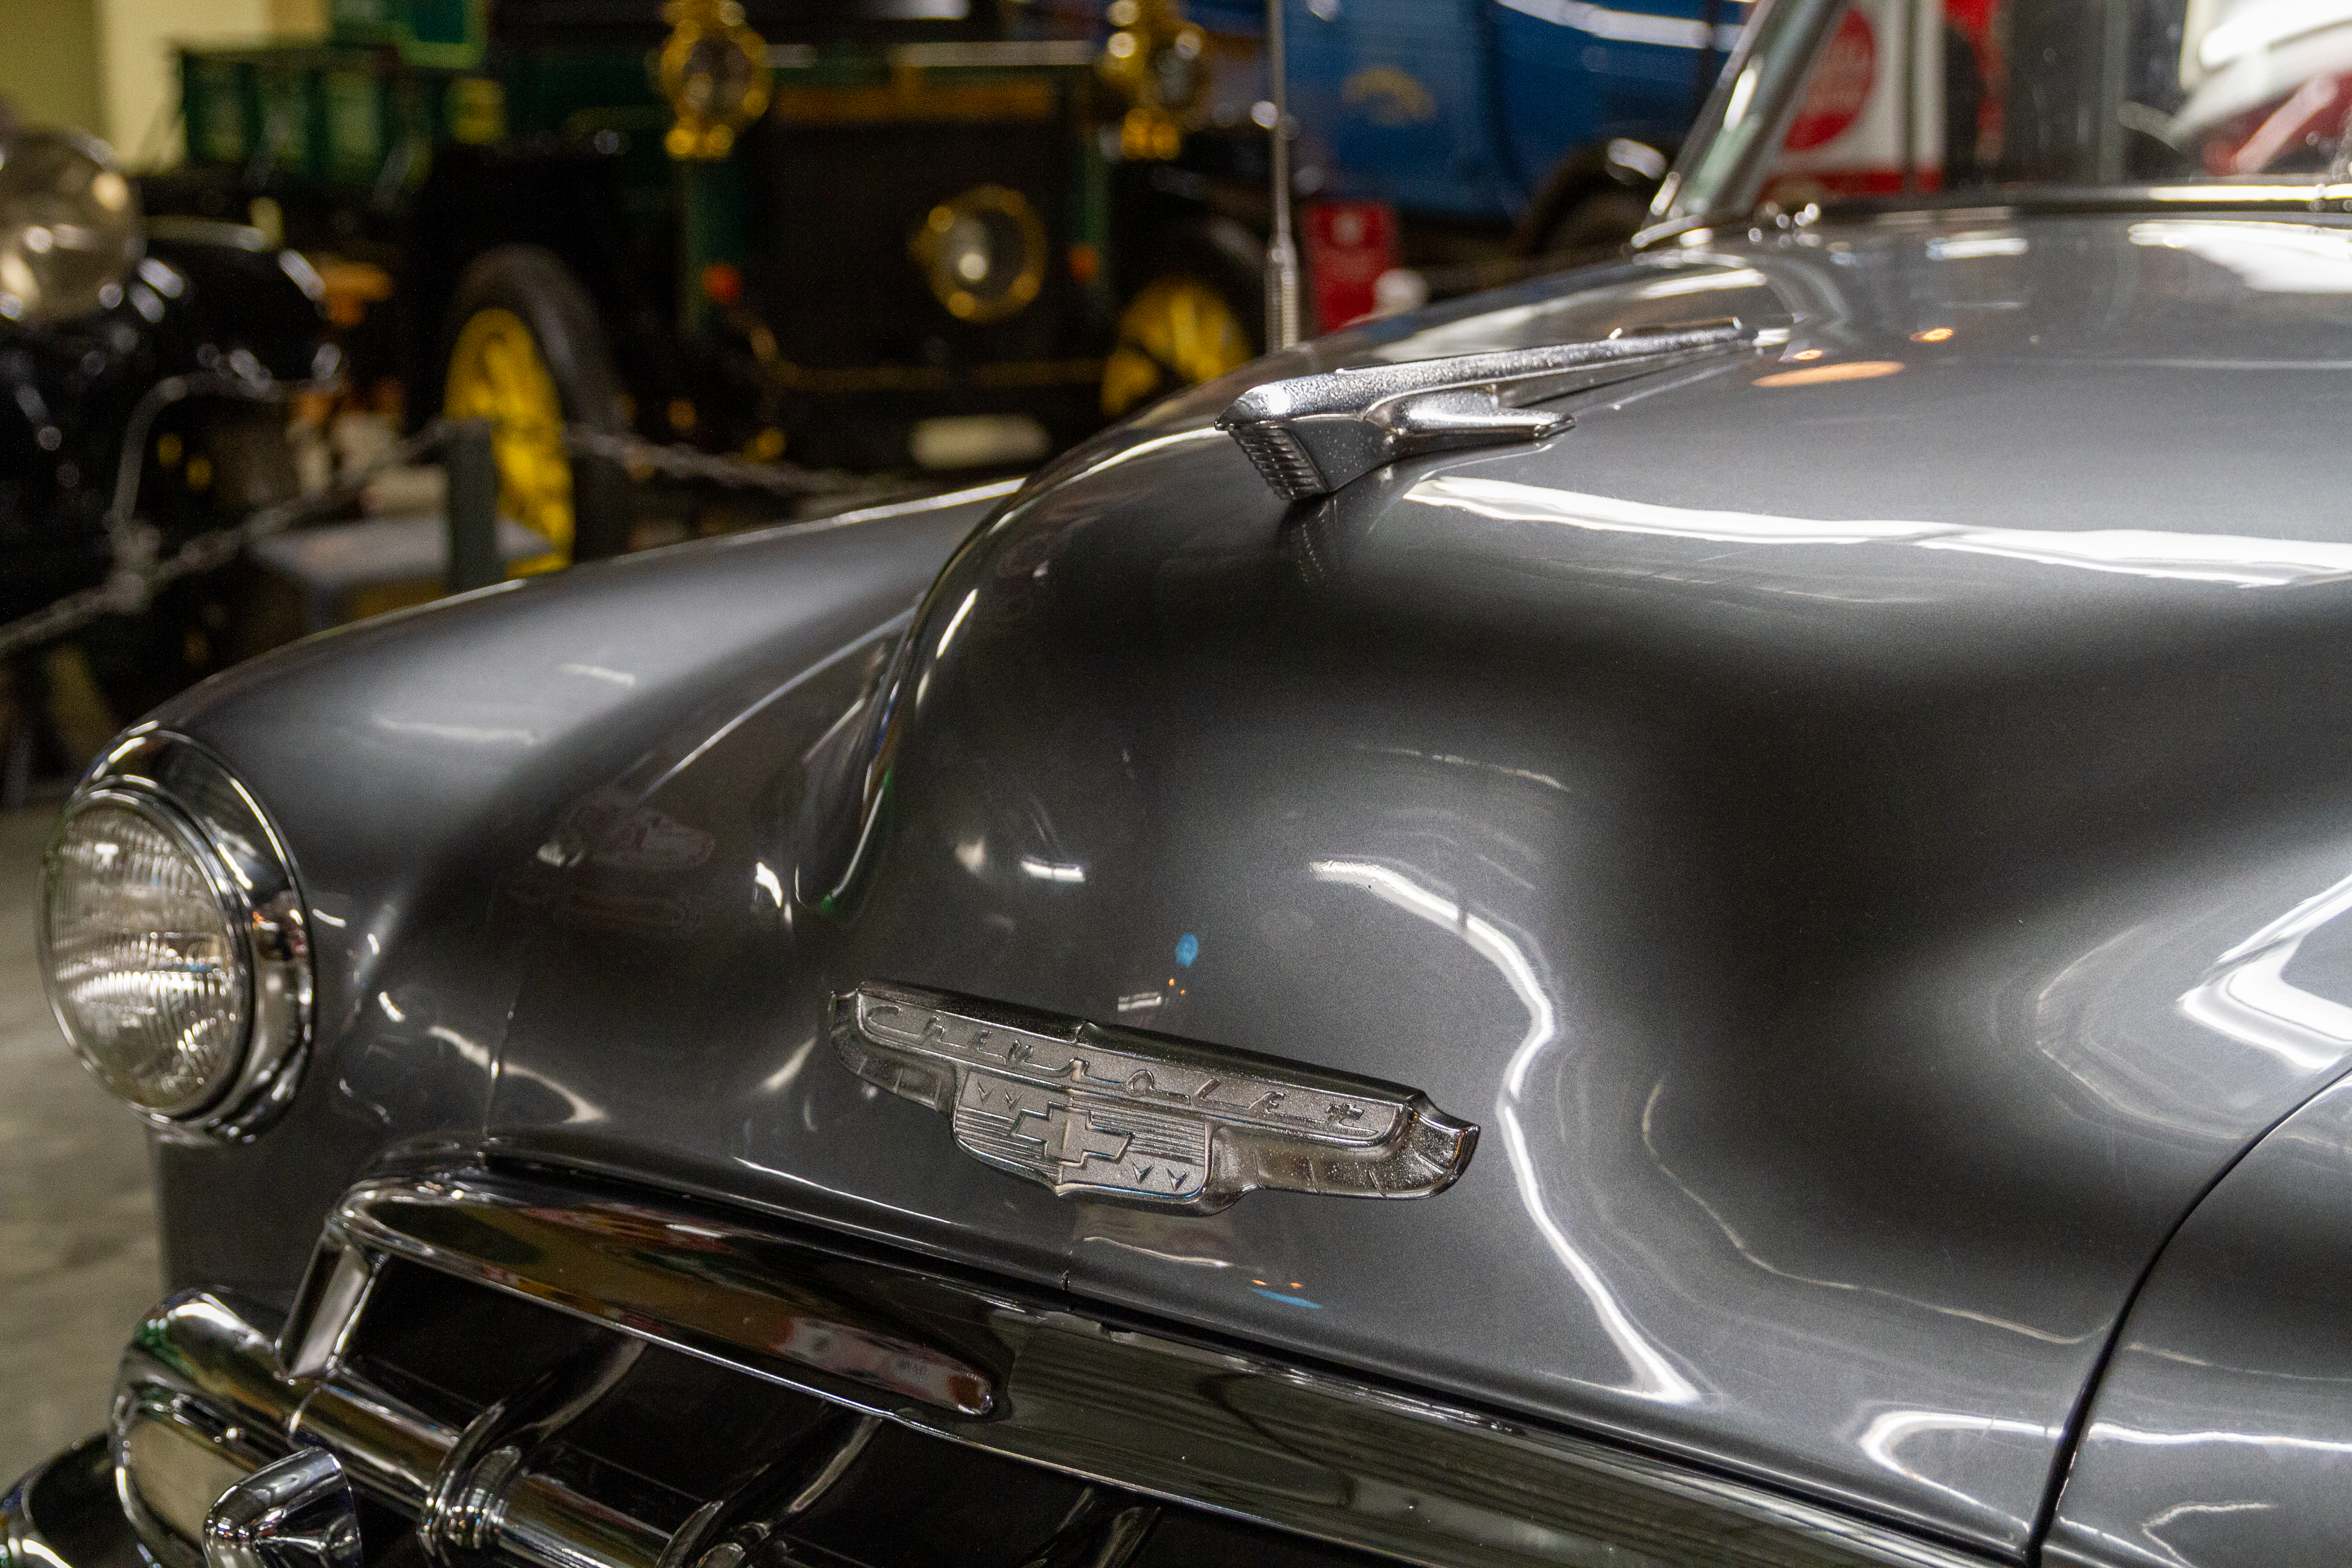
\includegraphics[width=0.6\textwidth]{example-image-a}
	\caption[Kurzer Titel fürs Abbildungsverzeichnis]{Ausführliche Bildunterschrift, die im Text erscheint}
	\label{fig:beispiel}
\end{figure}

\subsection{Zweites Grundlagenthema}
\label{cap:grundlage2}

\subsubsection{Unterpunkt}

Text.

\paragraph{Absatzüberschrift:}
Text.

% !TeX root = ../main.tex
\section{Methodik und Versuchsaufbau}
\label{cap:methodik}

Beschreibung des methodischen Vorgehens, der eingesetzten Messtechnik und der Versuchsplanung.

\subsection{Eingesetzte Messtechnik}
\label{cap:messtechnik}

Text.

\subsection{Versuchsplanung}
\label{cap:versuchsplanung}

Die wichtigsten Einstellungen sind:
\begin{itemize}
	\item Parameter 1: \SI{300}{\micro\metre}
	\item Parameter 2: \SI{50}{\micro\metre\per\second}
\end{itemize}

Ablauf einer Messung:
\begin{enumerate}[itemsep=0pt]
	\item Schritt 1
	\item Schritt 2
	\item Schritt 3
\end{enumerate}

% !TeX root = ../main.tex
\section{Ergebnisse}
\label{cap:ergebnisse}

Tabelle~\ref{tab:beispiel} zeigt eine Beispieltabelle im Stil der Bachelorarbeit.

\begin{table}[H]
	\centering
	\caption{Beispieltabelle mit an der Dezimalstelle ausgerichteten Zahlen}
	\label{tab:beispiel}
	\begin{tabular}{
			c
			S[table-format=1.3]
			S[table-format=2.2]
		}
		\toprule
		\textbf{Probe} & \textbf{Formparameter} & \textbf{Skalenparameter [\si{\newton}]} \\
		\midrule
		P1 & 5,849 & 38,27 \\
		P2 & 4,583 & 37,39 \\
		\bottomrule
	\end{tabular}
\end{table}

Abbildung~\ref{fig:vergleich} zeigt zwei Bilder nebeneinander.

\begin{figure}[H]
	\centering
	\begin{subfigure}{0.48\textwidth}
		\centering
		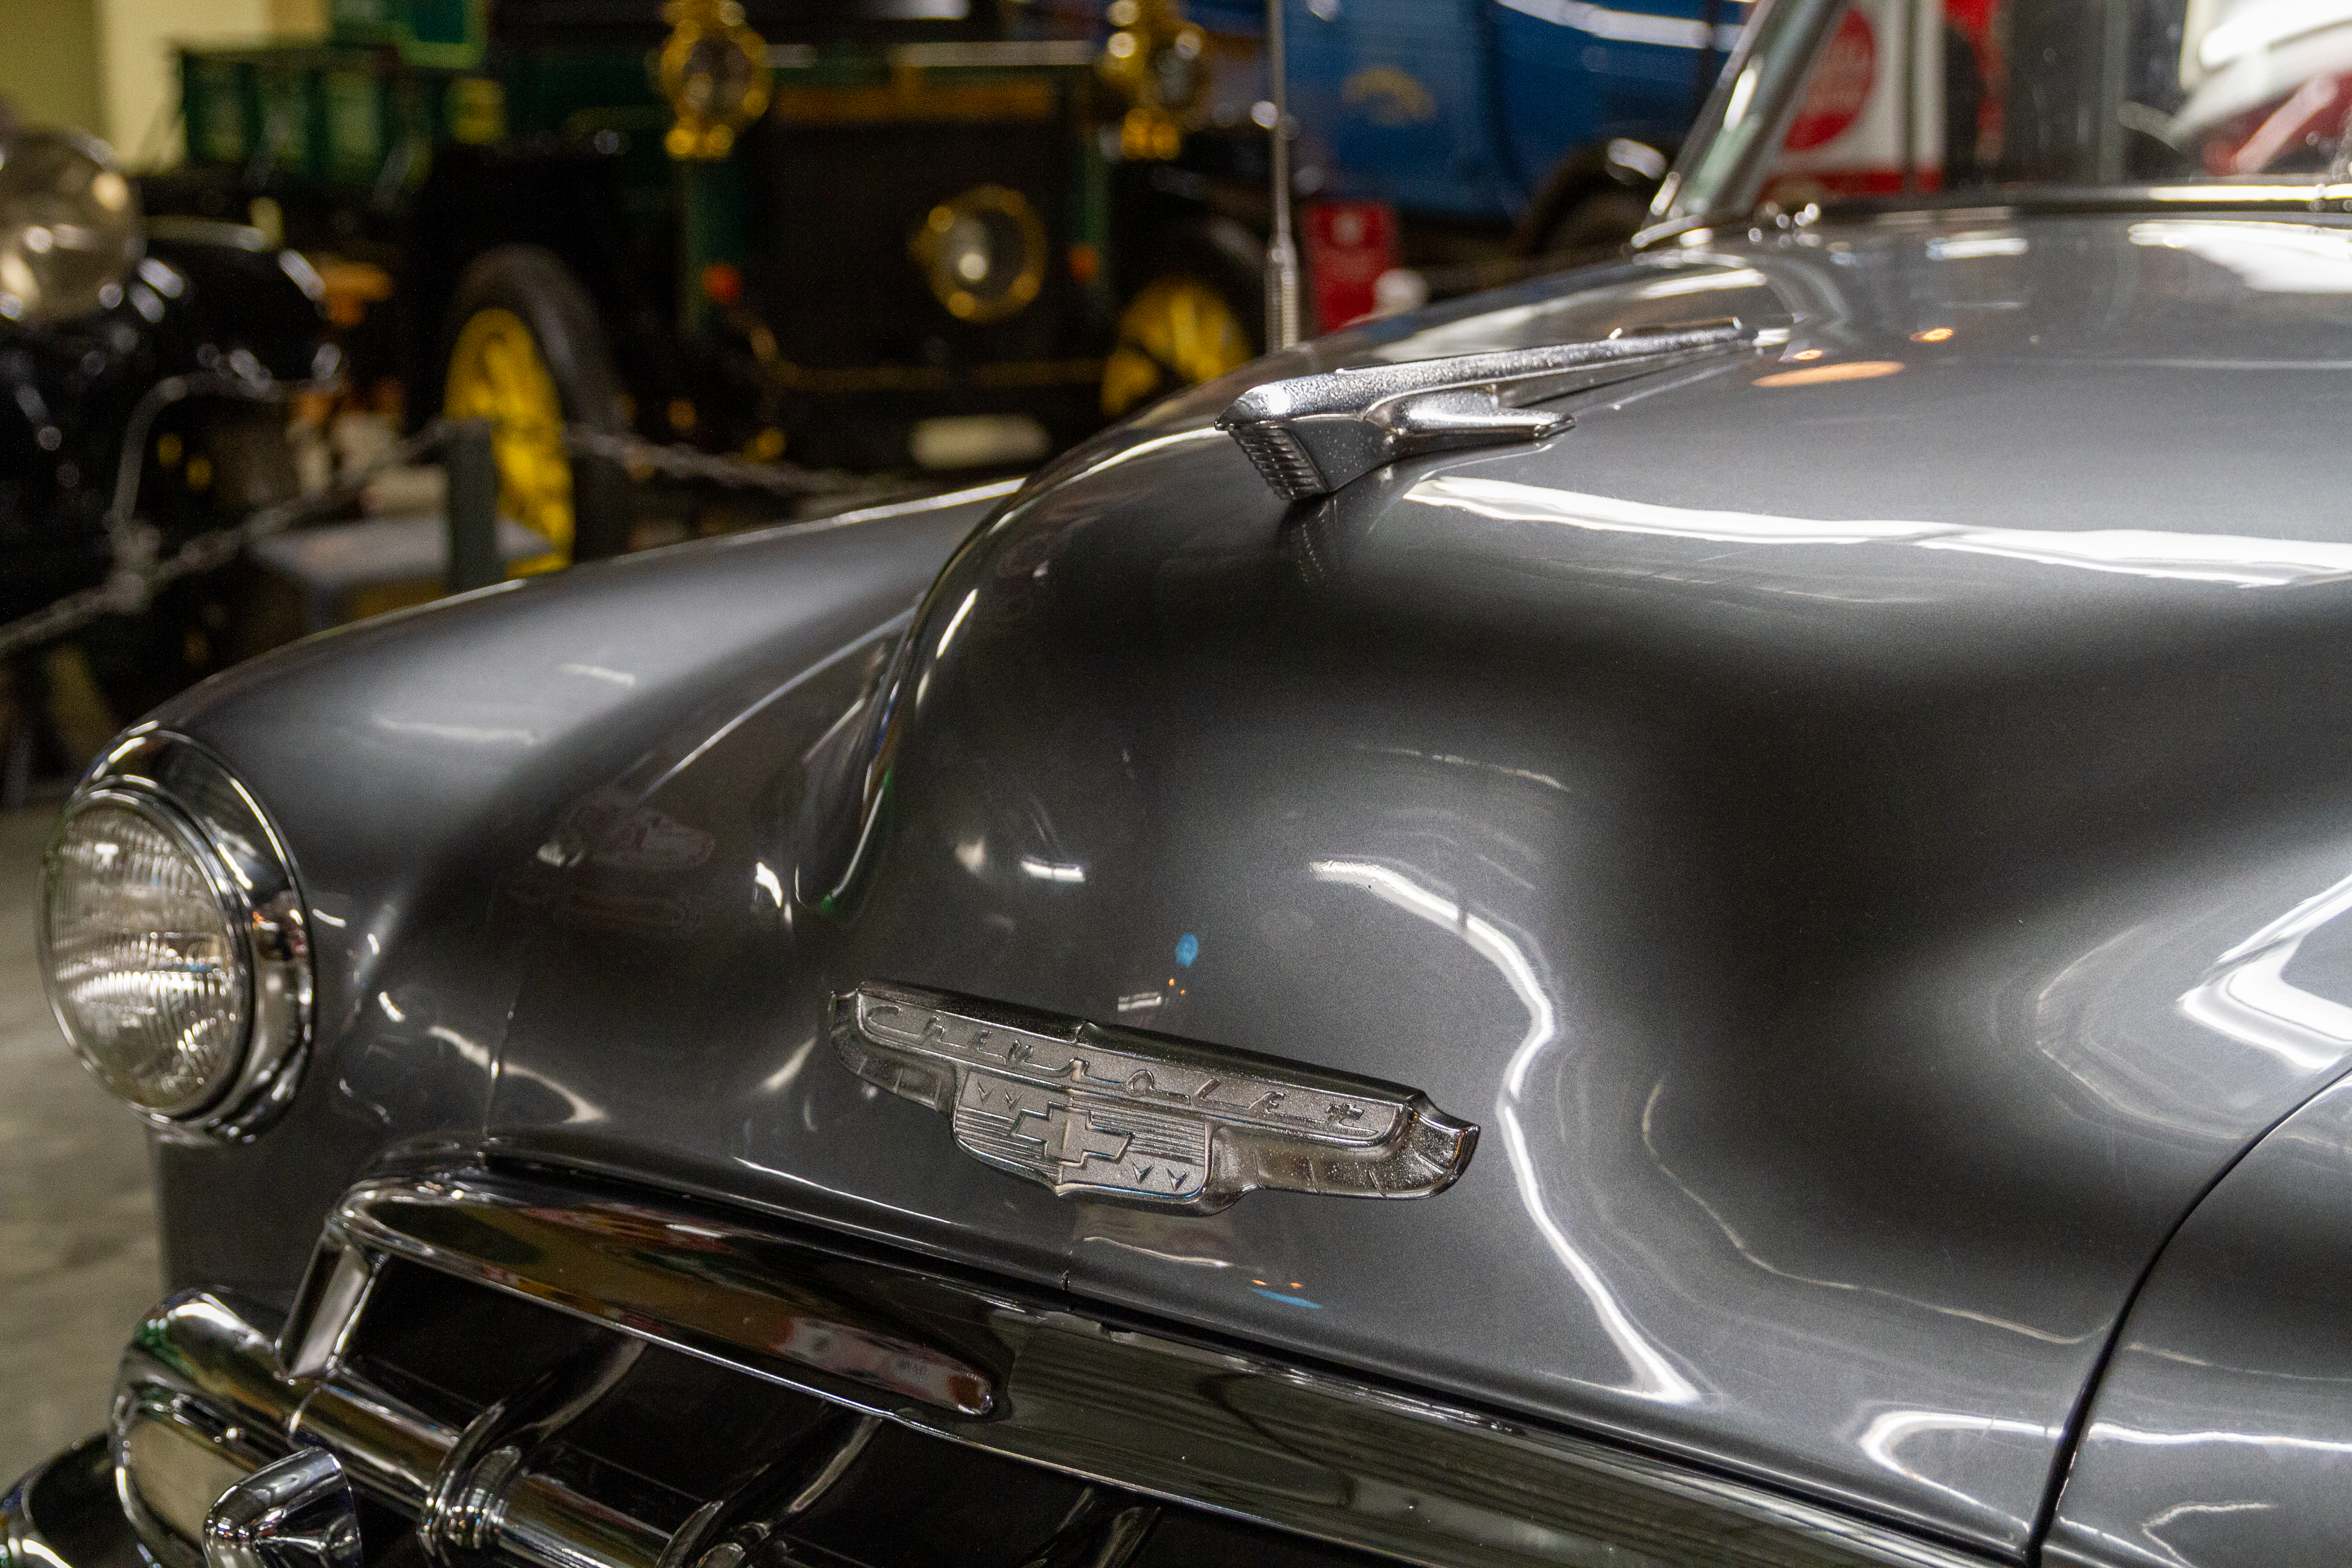
\includegraphics[width=\linewidth]{example-image-b}
		\caption{Variante A}
		\label{fig:vergleich_a}
	\end{subfigure}
	\hfill
	\begin{subfigure}{0.48\textwidth}
		\centering
		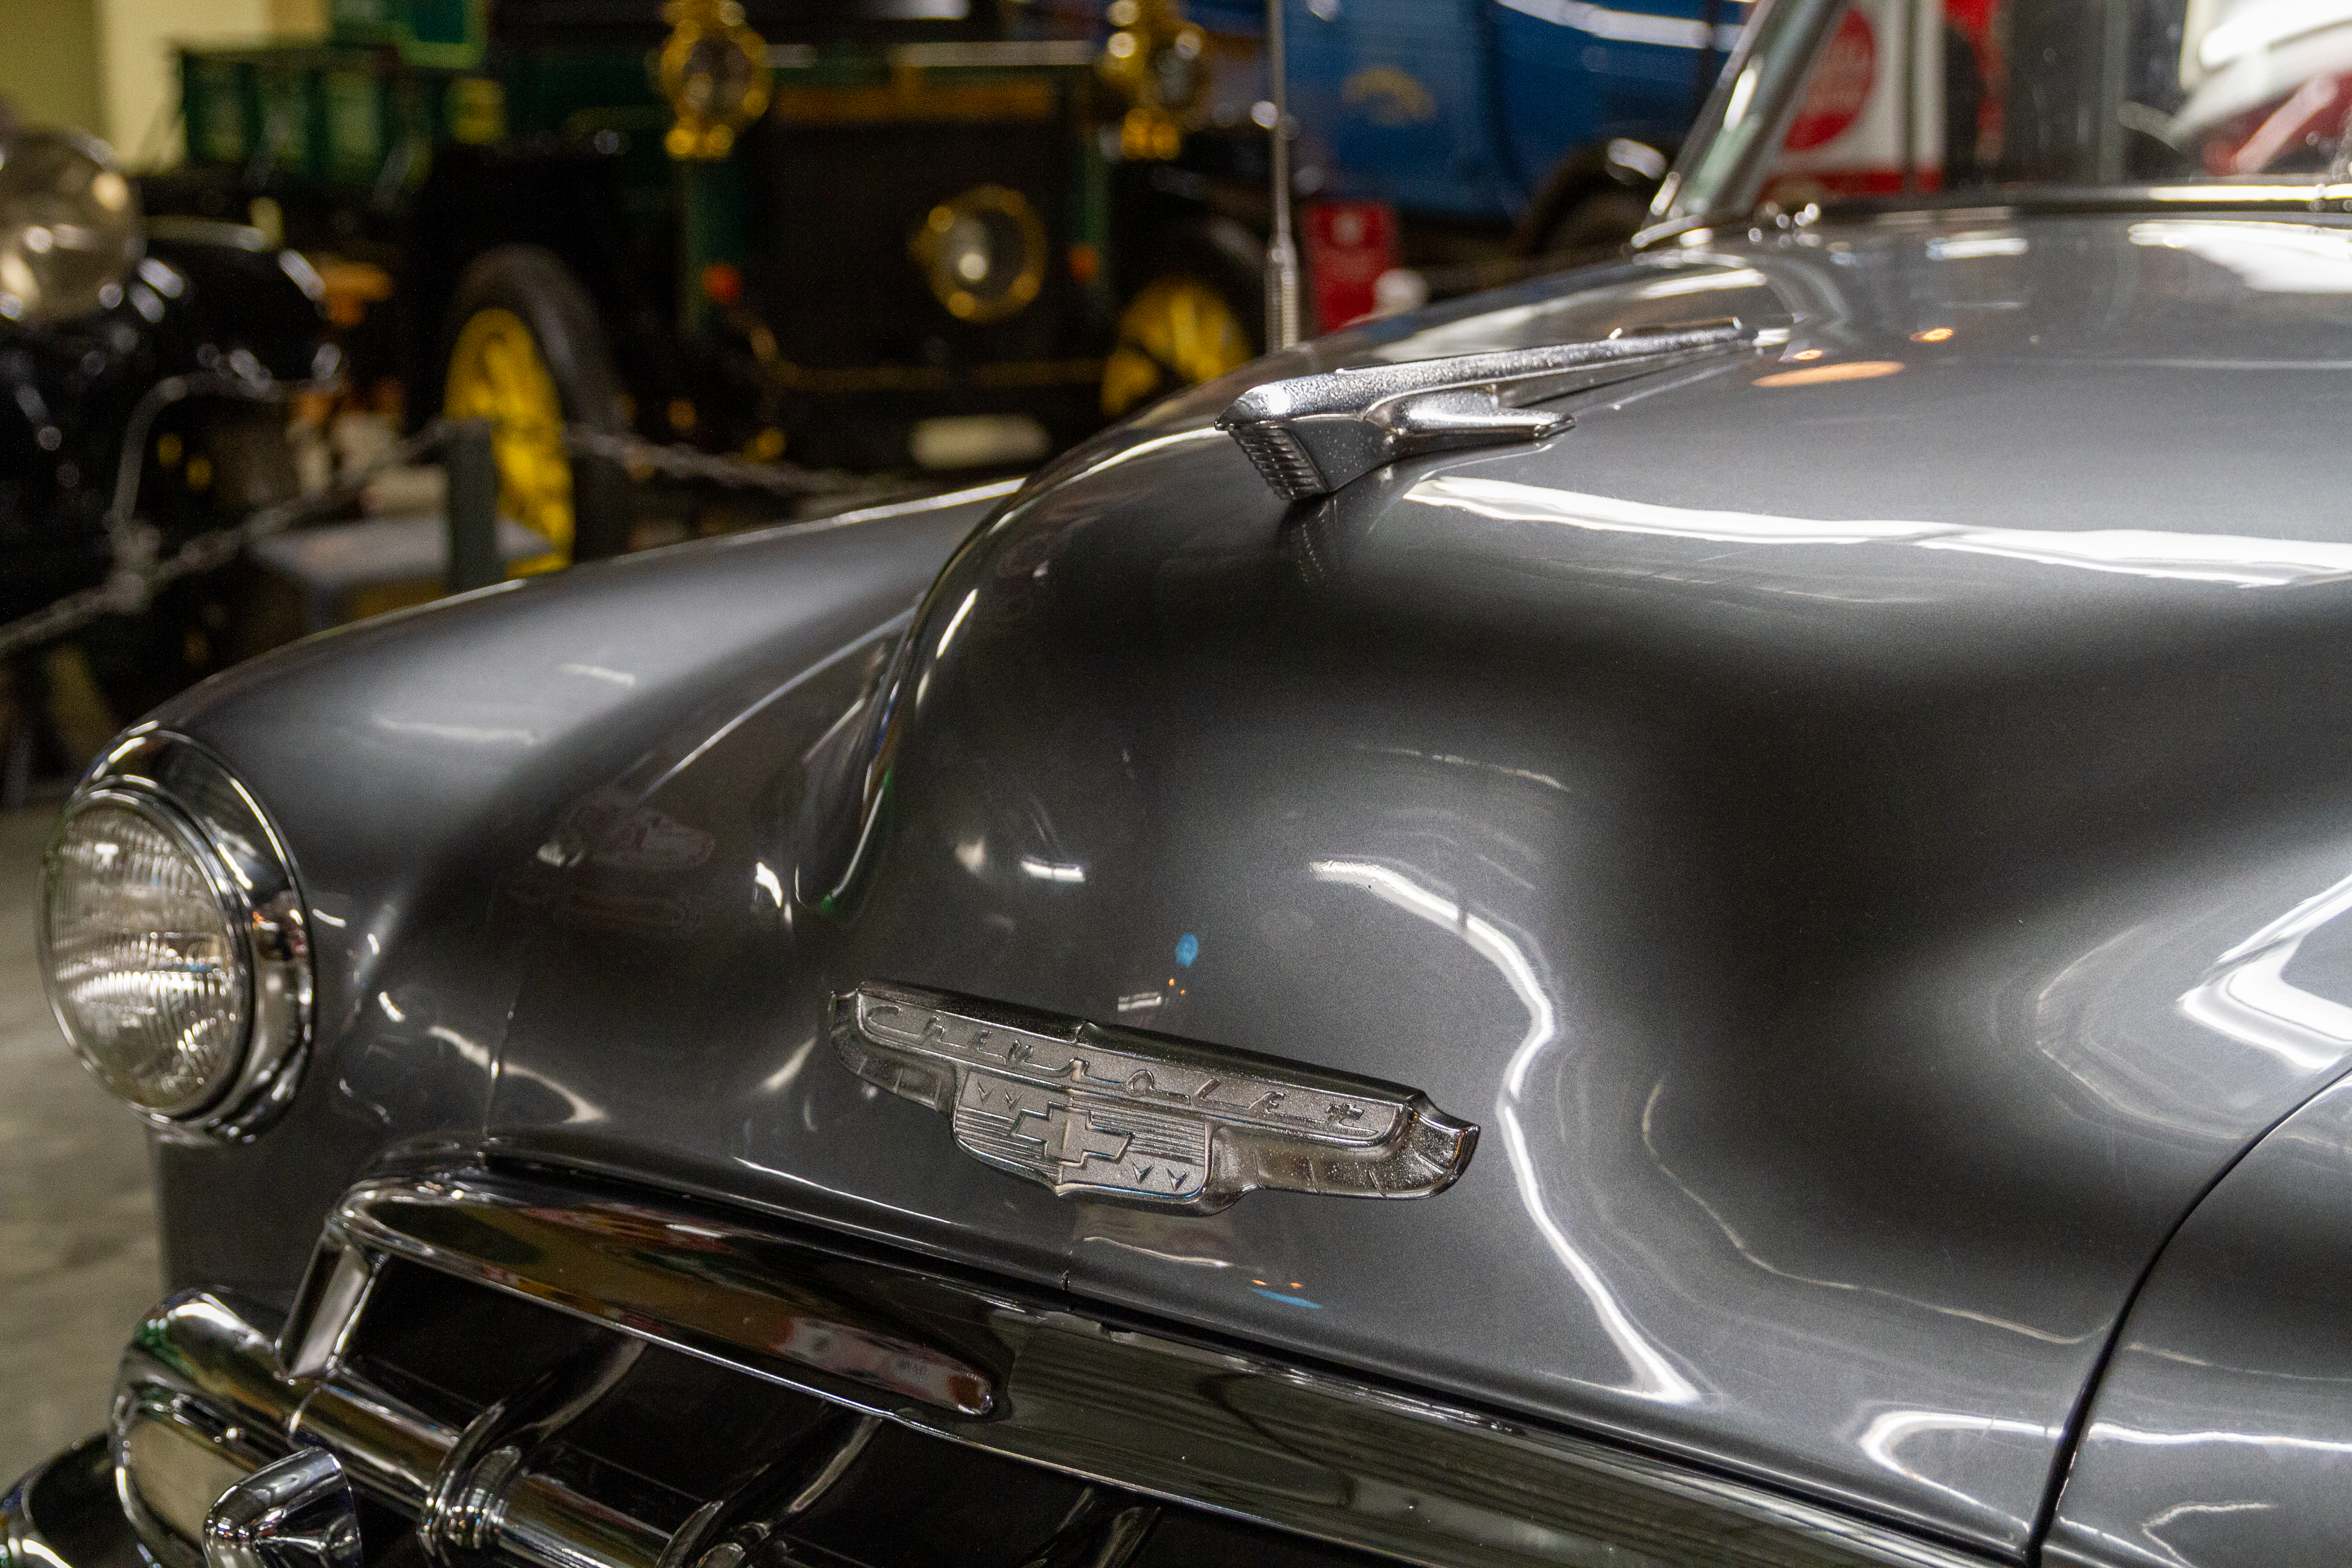
\includegraphics[width=\linewidth]{example-image-c}
		\caption{Variante B}
		\label{fig:vergleich_b}
	\end{subfigure}
	\caption{Vergleich zweier Varianten}
	\label{fig:vergleich}
\end{figure}

% !TeX root = ../main.tex
\section{Diskussion}
\label{cap:diskussion}

Einordnung und kritische Bewertung der Ergebnisse aus Kapitel~\ref{cap:ergebnisse}.

% !TeX root = ../main.tex
\section{Ausblick}
\label{cap:ausblick}

Offene Punkte und Ansätze für weiterführende Arbeiten.

% !TeX root = ../main.tex
\section{Fazit}
\label{cap:fazit}

Ziel dieser Arbeit war \dots
Beantwortung der Forschungsfragen aus Kapitel~\ref{cap:einleitung}.


% ========== Verzeichnisse (römisch, fortlaufend) ==========
\clearpage
\pagenumbering{Roman}
\setcounter{page}{\value{SeiteVorspann}}

\phantomsection
\addcontentsline{toc}{section}{Abbildungsverzeichnis}
\listoffigures
\newpage

\phantomsection
\addcontentsline{toc}{section}{Tabellenverzeichnis}
\listoftables
\newpage

% ========== Literaturverzeichnis ==========
\printbibliography[heading=bibintoc]
\newpage

% ========== Anhang (Seitenzahlen A, B, C ...) ==========
% !TeX root = ../main.tex
% ========= Anhang ==========================
\section*{Anhang}
\addcontentsline{toc}{section}{Anhang}
\appendix
\renewcommand{\thepage}{\Alph{page}} % Seitenzahlen als A, B, C
\setcounter{page}{1}

% Überschrift eines Anhangs im Stil der BA:  \anhangtitel{A: Titel}
\newcommand{\anhangtitel}[1]{\par\noindent{\large\textbf{Anhang #1}}\par}

\anhangtitel{A: Digitaler Anhang}
\label{page:digitaleAnhang}
\noindent Der digitale Anhang ist auf dem beiliegenden USB-Stick gespeichert.
Folgende Dateien sind in den Ordnern unter den angegebenen Dateipfaden zu finden:
\begin{itemize}
	\item Beschreibung: \\ \texttt{./Anhang(digital)/Ordnername}
\end{itemize}

\newpage
\anhangtitel{B: Weitere Abbildungen}
\label{page:AnhangB}
\begin{figure}[H]
	\centering
	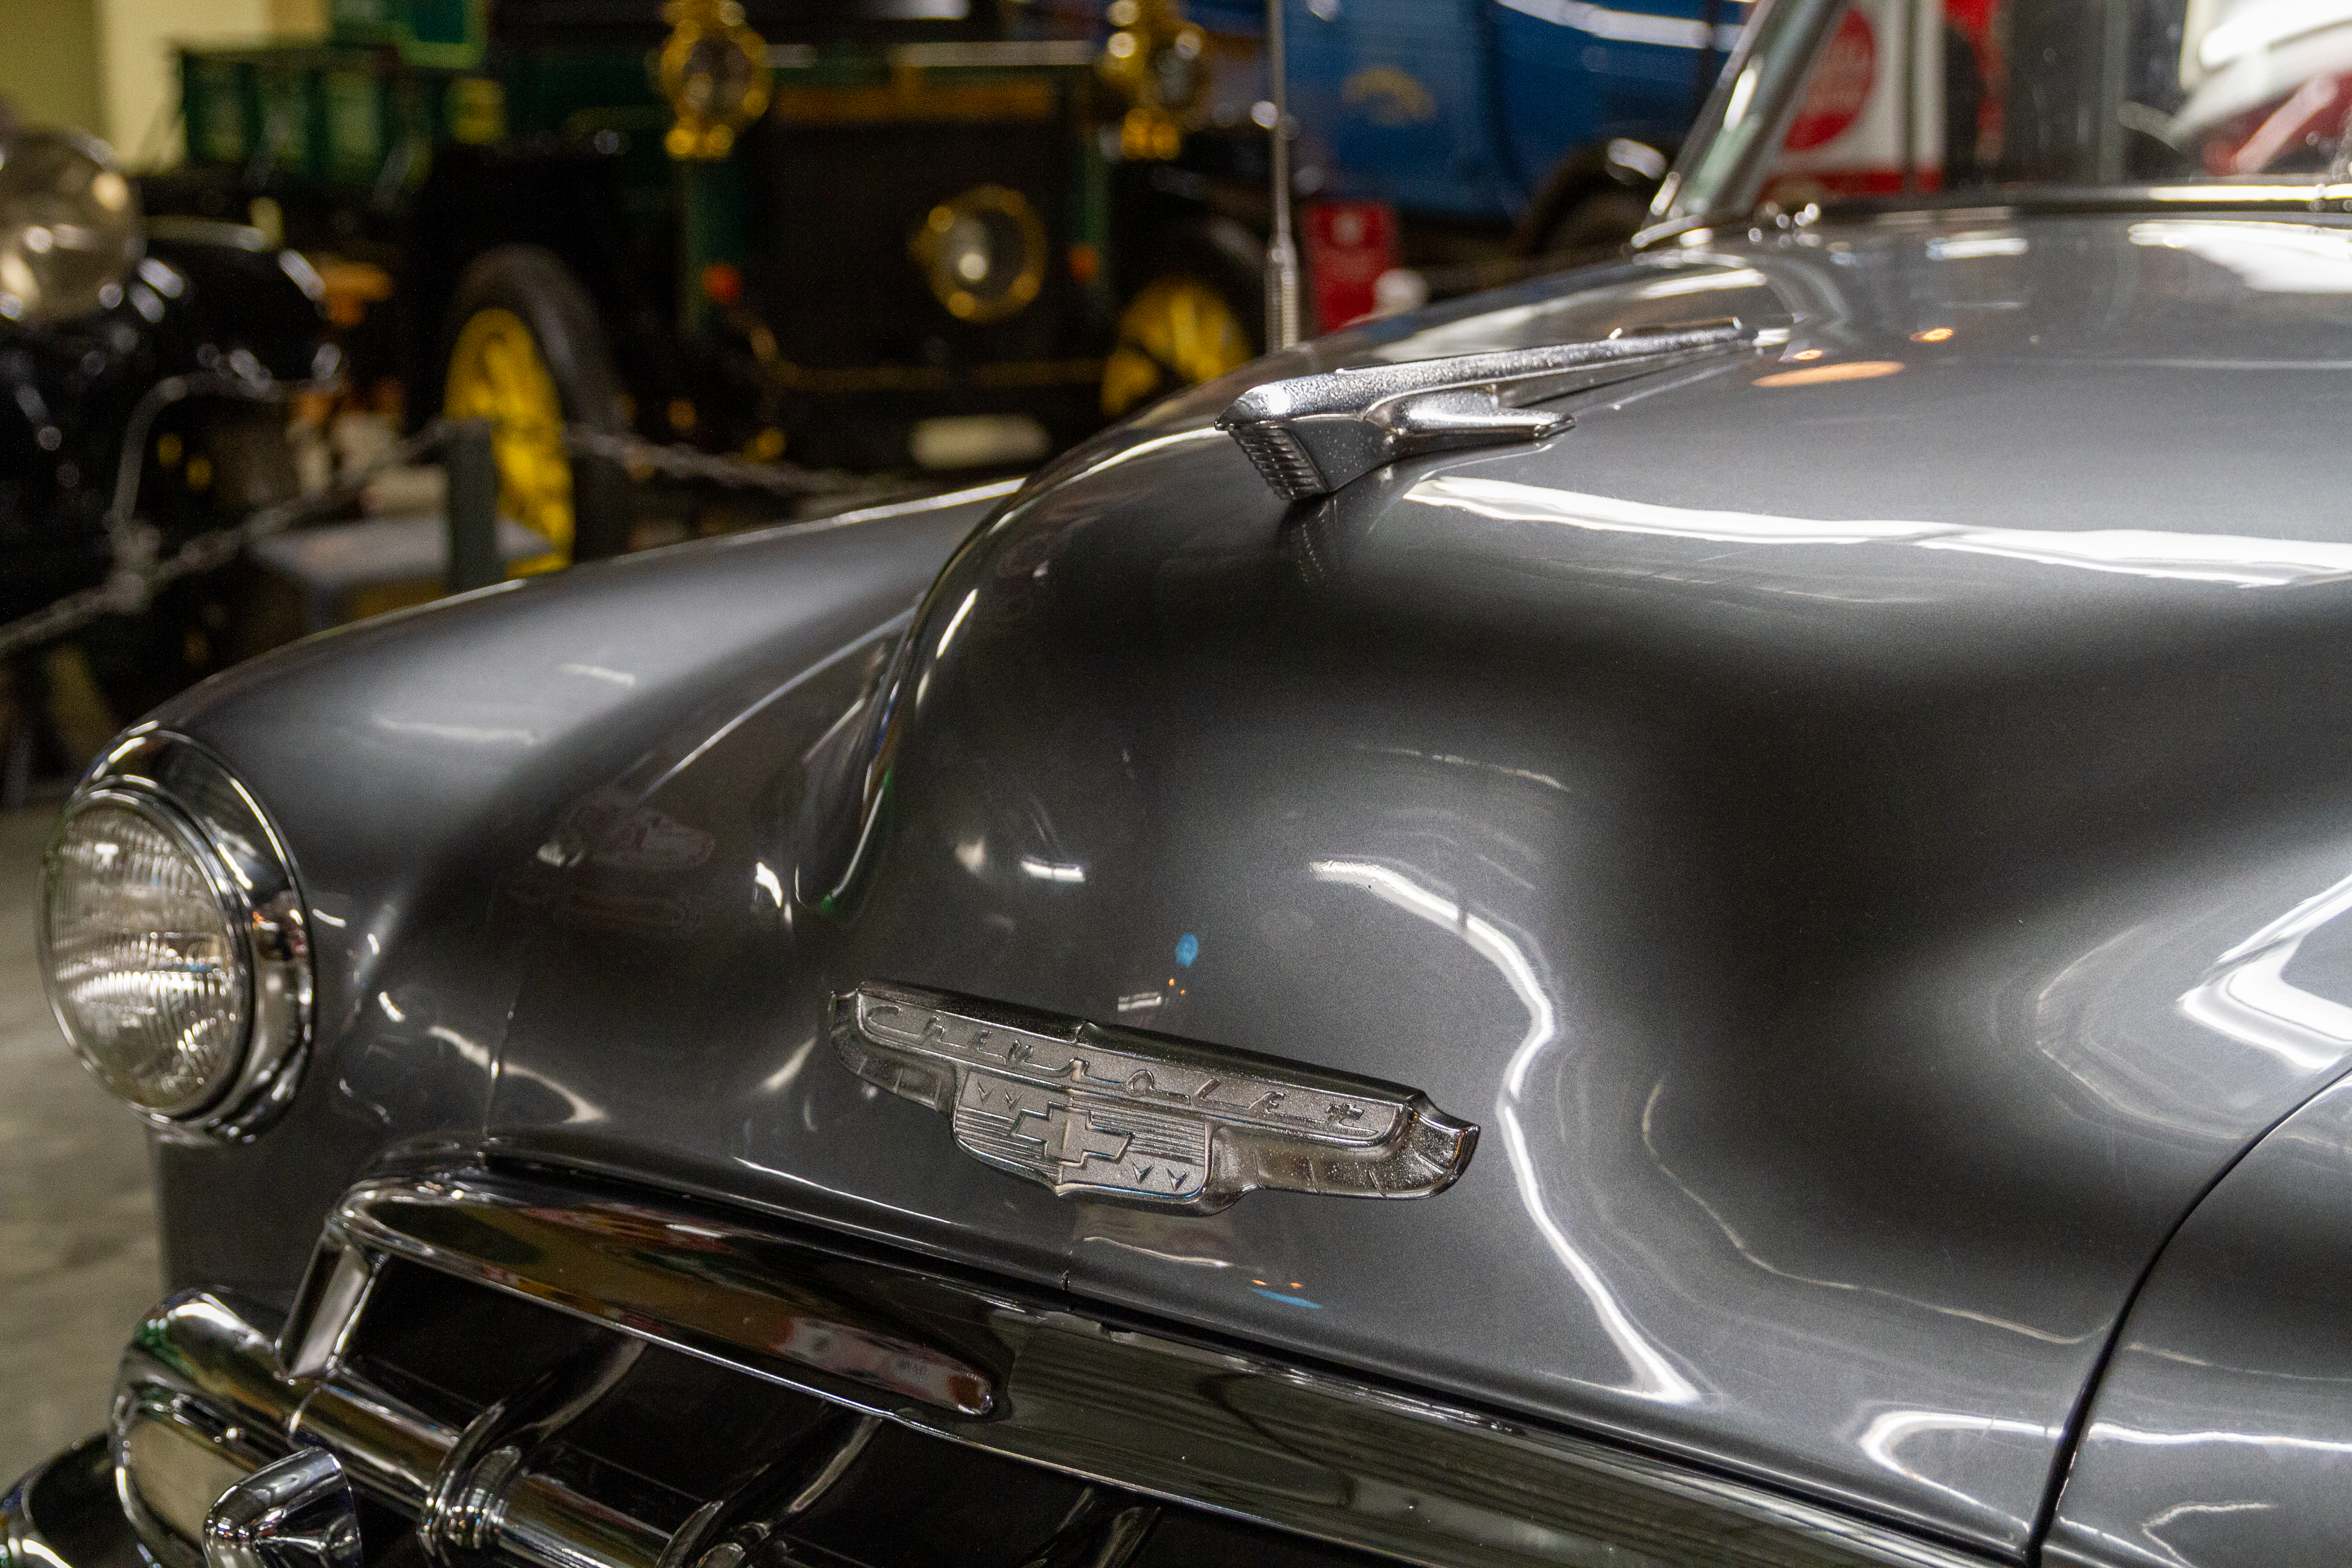
\includegraphics[width=0.6\textwidth]{example-image}
	\caption{Abbildung im Anhang}
	\label{fig:anhang_beispiel}
\end{figure}

% Externe PDF (z. B. Minitab-Bericht) einbinden:
% \newpage
% \includepdf[
%   pages=-,
%   scale=1.0,
%   offset=0 -15,
%   pagecommand={\thispagestyle{plain}\anhangtitel{C: Titel}}
% ]{./abbildungen/Anhang/Bericht.pdf}


\end{document}
